\section{Auswertung}
\label{sec:Auswertung}


\subsection{Ausmessung der Einfachspalte}

Die Breite der drei Einfachspalte wird auf zwei verschiedene Arten bestimmt.
Die Herstellerangaben betragen:
\begin{align*}
  b_\text{Spalt 1} &= \SI{0.075}{\milli\meter} & b_\text{Spalt 2} &= \SI{0.15}{\milli\meter} &
   b_\text{Spalt 3} &= \SI{0.4}{\milli\meter}.
\end{align*}

\subsubsection{Bestimmung der Breite mit Mikroskop}
\label{sec:einfachmikro}

Zunächst werden die Einfach-Spalte per Mikroskop ausgemessen.
Das in der Mikroskopanzeige eingebettete Kästchen wird bei 3.2-facher Vergrößerung
mit Hilfe einer geeichten Skala auf $3.2 \cdot \text{Square} = \SI{0.5}{\milli\meter}$ bestimmt.
Demnach beträgt die Größe des Kästchens:
\begin{equation*}
  \text{Square} = \SI{0.156}{\milli\meter}.
\end{equation*}
Per Dreisatz kann nun die Breite der Spalte durch vier-fache Vergrößerung
bestimmt werden.
Messwerte und Ergebnisse sowie der  Vergleich mit den Herstellerangaben $\Delta b$ finden sich
in Tabelle \ref{tab:mikroskopeinzel}.

\begin{table}[h]
  \centering
  %\begin{minipage}[t]{0.3\linewidth}
    \begin{tabular}{S S S S}
      \toprule
      {Spalt Nr.} & {$b_\text{mess} \:/\: 4\cdot \text{Square}$} & {$b_\text{mess}\:/\:\si{\milli\meter}$}
      & {$\Delta b\:/\:\si{\percent}$}\\
      \midrule
        1 & 1/7 & 0.089 & 19\\
        2 & 1/3 & 0.208 & 39\\
        3 & 1 & 0.625 & 56\\
      \bottomrule
    \end{tabular}
%  \end{minipage}
%  \begin{minipage}[t]{0.3\linewidth}
%  \end{minipage}
  \caption{Messwerte und Ergebnisse bei Bestimmung der Breite der Einfachspalte per Mikroskopmessung.}
  \label{tab:mikroskopeinzel}
\end{table}

\subsubsection{Bestimmung der Breite per Intensitätsmessung}

Nun werden die Spalte mit einem Laser bestrahlt und das Beugungsmuster aufgenommen.
Die Wellenlänge des Lasers und der Abstand von Spalt zur Beobachtungsebene betragen:
\begin{align*}
  \lambda &= \SI{633}{\nano\meter} & L &= \SI{1}{\meter}.
\end{align*}

Die Messwerte der Intensitätsmessung sind in den Tabellen \ref{tab:einzelspaltelinks} und \ref{tab:einzelspalterechts}
zu sehen. In den Graphen \ref{fig:einzelspalt1}, \ref{fig:einzelspalt2} und
\ref{fig:einzelspalt3} sind die Messwerte und die nach Gleichung \eqref{eqn:???}
durchgeführte Ausgleichsrechnung aufgetragen.

\begin{table}[h]
  \centering
  %\begin{minipage}[t]{0.3\linewidth}
    \begin{tabular}{S S S S}
      \toprule
      {$x-x_0 \:/\: \si{\milli\meter}$} & {$I_\text{Spalt 1}\:/\:\si{\micro\ampere}$} & {$I_\text{Spalt 2}\:/\:\si{\micro\ampere}$}
      & {$I_\text{Spalt 3}\:/\:\si{\micro\ampere}$}\\
      \midrule
      -14.5 & 6.8e-3 & 0.0175 & 0.012\\
      -14 & 9.6e-3 & 0.0185 & 0.015\\
      -13.5 & 0.0125 & 0.016 & 0.028\\
      -13 & 0.016 & 0.011 & 0.028\\
      -12.5 & 0.019 & 0.007 & 0.018\\
      -12 & 0.021 & 0.0072 & 0.033\\
      -11.5 & 0.0225 & 0.0115 & 0.041\\
      -11 & 0.023 & 0.0195 & 0.023\\
      -10.5 & 0.022 & 0.027 & 0.022\\
      -10 & 0.02 & 0.028 & 0.028\\
      -9.5 & 0.017 & 0.024 & 0.022\\
      -9 & 0.0135 & 0.0185 & 0.038\\
      -8.5 & 0.0105 & 0.012 & 0.051\\
      -8 & 0.009 & 0.0115 & 0.036\\
      -7.5 & 0.01 & 0.022 & 0.056\\
      -7 & 0.0145 & 0.041 & 0.081\\
      -6.5 & 0.0225 & 0.063 & 0.052\\
      -6 & 0.034 & 0.076 & 0.075\\
      -5.5 & 0.052 & 0.072 & 0.125\\
      -5 & 0.076 & 0.05 & 0.06\\
      -4.5 & 0.1 & 0.027 & 0.105\\
      -4 & 0.13 & 0.023 & 0.235\\
      -3.5 & 0.165 & 0.07 & 0.175\\
      -3 & 0.2 & 0.21 & 0.26\\
      -2.5 & 0.235 & 0.42 & 0.68\\
      -2 & 0.27 & 0.76 & 0.68\\
      -1.5 & 0.27 & 1.05 & 1.3\\
      -1 & 0.3 & 1.45 & 6.6\\
      -0.5 & 0.32 & 1.75 & 15\\
      \bottomrule
    \end{tabular}
%  \end{minipage}
%  \begin{minipage}[t]{0.3\linewidth}
%  \end{minipage}
  \caption{Intensitätsamplitude der drei Einzelspalte(links von $x_0$).}
  \label{tab:einzelspaltelinks}
\end{table}

\begin{table}[h]
  \centering
  %\begin{minipage}[t]{0.3\linewidth}
%  \end{minipage}
%  \begin{minipage}[t]{0.3\linewidth}
    \begin{tabular}{S S S S}
      \toprule
      {$x-x_0 \:/\: \si{\milli\meter}$} & {$I_\text{Spalt 1}\:/\:\si{\micro\ampere}$} & {$I_\text{Spalt 2}\:/\:\si{\micro\ampere}$}
      & {$I_\text{Spalt 3}\:/\:\si{\micro\ampere}$}\\
      \midrule
      0 & 0.33 & 1.8 & 20\\
      0.5 & 0.31 & 1.8 & 14\\
      1 & 0.31 & 1.6 & 4.5\\
      1.5 & 0.29 & 1.3 & 0.85\\
      2 & 0.27 & 0.95 & 0.65\\
      2.5 & 0.24 & 0.66 & 0.65\\
      3 & 0.21 & 0.35 & 0.26\\
      3.5 & 0.18 & 0.18 & 0.21\\
      4 & 0.16 & 0.072 & 0.26\\
      4.5 & 0.13 & 0.044 & 0.13\\
      5 & 0.095 & 0.058 & 0.13\\
      5.5 & 0.07 & 0.084 & 0.16\\
      6 & 0.053 & 0.095 & 0.08\\
      6.5 & 0.036 & 0.09 & 0.07\\
      7 & 0.024 & 0.078 & 0.09\\
      7.5 & 0.017 & 0.055 & 0.06\\
      8 & 0.013 & 0.034 & 0.045\\
      8.5 & 0.0135 & 0.026 & 0.065\\
      9 & 0.0145 & 0.0255 & 0.045\\
      9.5 & 0.016 & 0.028 & 0.03\\
      10 & 0.019 & 0.034 & 0.04\\
      10.5 & 0.021 & 0.034 & 0.035\\
      \bottomrule
    \end{tabular}
%  \end{minipage}
  \caption{Intensitätsamplitude der drei Einzelspalte(rechts von $x_0$).}
  \label{tab:einzelspalterechts}
\end{table}

\begin{figure}
  \centering
  \includegraphics[width = \textwidth]{build/einzelspalt1.pdf}
  \caption{Messwerte und Ausgleichsrechnung zu Spalt 1.}
  \label{fig:einzelspalt1}
\end{figure}

\begin{figure}
  \centering
  \includegraphics[width = \textwidth]{build/einzelspalt2.pdf}
  \caption{Messwerte und Ausgleichsrechnung zu Spalt 2.}
  \label{fig:einzelspalt2}
\end{figure}

\begin{figure}
  \centering
  \includegraphics[width = \textwidth]{build/einzelspalt3.pdf}
  \caption{Messwerte und Ausgleichsrechnung zu Spalt 3.}
  \label{fig:einzelspalt3}
\end{figure}

Die bestimmten Breiten und die Abweichung von der Herstellerangabe, die die Ausgleichsrechnung
ergibt, sind in Tabelle
\ref{tab:ergeinzelint} abzulesen.

\begin{table}[h]
  \centering
  \begin{tabular}{S
    S[table-format=1.4]
    @{${}\pm{}$}
    S[table-format=1.4]
    S[table-format=2.2]
    @{${}\pm{}$}
    S[table-format=1.1]
    S}
    \toprule
    {Spalt Nr.} & \multicolumn{2}{c}{$b_\text{mess}\:/\:\si{\milli\meter}$}
    & \multicolumn{2}{c}{$A_{0, \text{mess}}\:/\:\si{\ampere\per\meter}$}
    & {$\Delta b\:/\:\si{\percent}$}\\
    \midrule
      1 & 0.0750 & 0.0008 & 7.51 & 7 & 0.05\\
      2 & 0.146 & 0.002 & 9.3 & 0.1 & 2.9\\
      3 & 0.361 & 0.005 & 12.1 & 0.1 & 9.8\\
    \bottomrule
  \end{tabular}
  \caption{Die, sich aus der Ausgleichsrechnung ergebenden, Fitparameter.}
  \label{tab:ergeinzelint}
\end{table}

\FloatBarrier

\subsection{Ausmessung der Doppelspalte}

Die Herstellerangaben des Doppelspalts betragen:
\begin{align*}
  b &= \SI{0.1}{\milli\meter}\text{~~~~} a = \SI{0.4}{\milli\meter}.
\end{align*}
Wobei $b$ die Spaltbreite ist und $a$ den Abstand beider Spalte angibt.
Somit beträgt:
\begin{equation*}
  s = b + a = \SI{0.5}{\milli\meter}.
\end{equation*}

\subsubsection{Bestimmung der Parameter mit Mikroskop}

Die Mikroskopmessung verläuft genauso wie in Kapitel \ref{sec:einfachmikro}.
Die Ergebnisse sind:
\begin{align*}
  b_\text{mess} &= 4 \cdot 0.23 \text{ Square} & a_\text{mess} &= 4\cdot 12/13 \text{ Square}\\
  b_\text{mess} &= \SI{0.144}{\milli\meter} & a_\text{mess} &= \SI{0.577}{\milli\meter}\\
  \Delta b &= \SI{43.8}{\percent} & \Delta a &= \SI{44.2}{\percent}.
\end{align*}
Demnach ist $s$:
\begin{align*}
  s &= \SI{0.721}{\milli\meter} & \Delta s &= \SI{44.1}{\percent}
\end{align*}

\subsubsection{Bestimmung der Parameter per Intensitätsmessung}

\begin{table}[h]
  \centering
  \begin{minipage}[t]{0.4\linewidth}
%  \end{minipage}
    \begin{tabular}{S[table-format=3.2]
      S[table-format=1.3]}
      \toprule
      {$x-x_0 \:/\: \si{\milli\meter}$} & {$I_\text{Doppelspalt}\:/\:\si{\micro\ampere}$}\\
      \midrule
      -11.25 & 0.029\\
      -11 & 0.03\\
      -10.75 & 0.046\\
      -10.5 & 0.075\\
      -10.25 & 0.091\\
      -10 & 0.083\\
      -9.75 & 0.074\\
      -9.5 & 0.088\\
      -9.25 & 0.12\\
      -9 & 0.145\\
      -8.75 & 0.135\\
      -8.5 & 0.1\\
      -8.25 & 0.09\\
      -8 & 0.11\\
      -7.75 & 0.13\\
      -7.5 & 0.12\\
      -7.25 & 0.08\\
      -7 & 0.06\\
      -6.75 & 0.06\\
      -6.5 & 0.075\\
      -6.25 & 0.075\\
      -6 & 0.06\\
      -5.75 & 0.075\\
      -5.5 & 0.135\\
      -5.25 & 0.205\\
      -5 & 0.22\\
      -4.75 & 0.21\\
      -4.5 & 0.275\\
      -4.25 & 0.46\\
      -4 & 0.68\\
      -3.75 & 0.76\\
      -3.5 & 0.67\\
      -3.25 & 0.72\\
      -3 & 1\\
      -2.75 & 1.5\\
      -2.5 & 1.65\\
      -2.25 & 1.4\\
      -2 & 1.3\\
      -1.75 & 1.65\\
      -1.5 & 2.3\\
      -1.25 & 2.6\\
    \end{tabular}
  \end{minipage}
\begin{minipage}[t]{0.4\linewidth}
  \begin{tabular}{S[table-format=2.2]
    S[table-format=1.3]}
    \toprule
    {$x-x_0 \:/\: \si{\milli\meter}$} & {$I_\text{Doppelspalt}\:/\:\si{\micro\ampere}$}\\
    \midrule
    -1 & 2.25\\
    -0.75 & 1.85\\
    -0.5 & 2\\
    -0.25 & 2.7\\
    0 & 2.8\\
    0.25 & 2.5\\
    0.5 & 1.9\\
    0.75 & 1.8\\
    1 & 2.2\\
    1.25 & 2.5\\
    1.5 & 2.2\\
    1.75 & 1.5\\
    2 & 1.2\\
    2.25 & 1.4\\
    2.5 & 1.6\\
    2.75 & 1.4\\
    3 & 1\\
    3.25 & 0.6\\
    3.5 & 0.75\\
    3.75 & 0.75\\
    4 & 0.7\\
    4.25 & 0.45\\
    4.5 & 0.3\\
    4.75 & 0.26\\
    5 & 0.23\\
    5.25 & 0.18\\
    5.5 & 0.14\\
    5.75 & 0.09\\
    6 & 0.08\\
    6.25 & 0.07\\
    6.5 & 0.045\\
    6.75 & 0.038\\
    7 & 0.051\\
    7.25 & 0.083\\
    7.5 & 0.105\\
    7.75 & 0.095\\
    8 & 0.075\\
    8.25 & 0.075\\
    8.5 & 0.1\\
    8.75 & 0.13\\
  \end{tabular}
\end{minipage}
  \caption{Messwerte bei der Intensitätsmessung am Doppelspalt.}
  \label{tab:doppelspalt}
\end{table}

In Tabelle \ref{tab:doppelspalt} sind die Messwerte der Intensitätsmessung
am Doppelspalt eingetragen. Mit Formel \eqref{eqn:???} wird dann eine Ausgleichsrechnung
durchgeführt. Allerdings wurde anstelle des Faktors "4" ein weiterer Fitparameter
"$A_0$" eingeführt, um die Ausgangsamplitude zu berücksichtigen. Die Messwerte und die Ausgleichsrechnung sind in Abbildung
\ref{fig:doppelspalt} abgebildet.

\begin{figure}
  \centering
  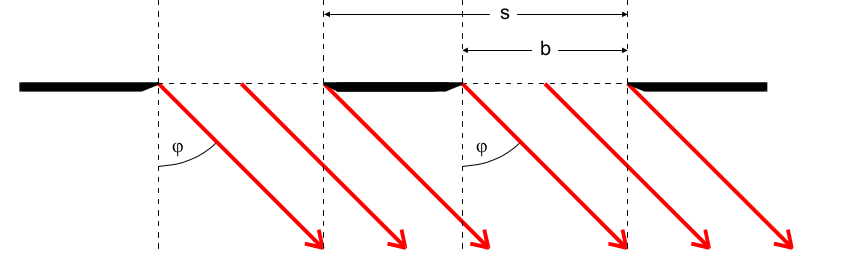
\includegraphics[width = \textwidth]{build/doppelspalt.pdf}
  \caption{Messwerte und Ausgleichsrechnung zum Doppelspalt.}
  \label{fig:doppelspalt}
\end{figure}

Die Ergebnisse aus der Ausgleichsrechnung sind:
 %Ergebnisse einfügen
\begin{align*}
  A_0 &=  \SI{3.681}{\micro\ampere} & &\\
  s &= \SI{0.483(6)}{\milli\meter} & \Delta s &= \SI{3.5}{\percent}\\
  b &= \SI{0.101(6)}{\milli\meter} & \Delta b &= \SI{1.1}{\percent}
\end{align*}

\subsubsection{Vergleich der Verteilungsbilder}

In Abbildung \ref{fig:vergleich} wurden alle vier in diesem Versuch bestimmten Intensitätsprofile zum Vergleich übereinander
gelegt.

\begin{figure}
  \centering
  \includegraphics[width = \textwidth]{build/vergleich.pdf}
  \caption{Vergleich der vier Intensitätsprofile.}
  \label{fig:vergleich}
\end{figure}

Einfachspalt Nr. 3 ist nicht ganz abgebildet, da die anderen Profile dann schwerer
erkennbar wären.
